\documentclass{article}


% if you need to pass options to natbib, use, e.g.:
%     \PassOptionsToPackage{numbers, compress}{natbib}
% before loading neurips


% ready for submission
% \usepackage{neurips}


% to compile a preprint version, e.g., for submission to arXiv, add add the
% [preprint] option:
    % \usepackage[preprint]{neurips}


% to compile a camera-ready version, add the [final] option, e.g.:
    \usepackage[final]{neurips}


% to avoid loading the natbib package, add option nonatbib:
%    \usepackage[nonatbib]{neurips}


\usepackage[utf8]{inputenc} % allow utf-8 input
\usepackage[T1]{fontenc}    % use 8-bit T1 fonts
\usepackage{hyperref}       % hyperlinks
\usepackage{url}            % simple URL typesetting
\usepackage{booktabs}       % professional-quality tables
\usepackage{amsfonts}       % blackboard math symbols
\usepackage{amsmath}        % math
\usepackage{subfigure}      % subfigures
\usepackage{graphicx}       % figures
\usepackage{nicefrac}       % compact symbols for 1/2, etc.
\usepackage{microtype}      % microtypography
\usepackage{xcolor}         % colors

\graphicspath{{resources}}


\title{Path Connectedness For Pixelwise Image Segmentation}


% The \author macro works with any number of authors. There are two commands
% used to separate the names and addresses of multiple authors: \And and \AND.
%
% Using \And between authors leaves it to LaTeX to determine where to break the
% lines. Using \AND forces a line break at that point. So, if LaTeX puts 3 of 4
% authors names on the first line, and the last on the second line, try using
% \AND instead of \And before the third author name.


\author{%
  Abdul-Karym Ismail \\
  University Siegen\\
  \texttt{abdul-karym.ismail@student.uni-siegen.de} \\
  % examples of more authors
  \And
  Prof. Dr. Michael Moeller \\
  University Siegen\\
  \texttt{michael.moeller@uni-siegen.de} \\
}


\begin{document}
\bibliographystyle{plainnat}


\maketitle

\begin{abstract}
    This research paper introduces a new machine learning technique for accurate per-pixel
    image segmentation. By incorporating the path-connectedness constraint,
    the model's output becomes more interpretable and robust against noise interference.
\end{abstract}

\section{Introduction}

The domain of image segmentation has witnessed significant advancements thanks to the utilization of deep learning techniques.
Deep learning provides a powerful approach to effectively capture and understand the underlying connections within the training data,
thereby generating high-quality segmentation masks across a wide range of datasets.
However, it is important to acknowledge that deep neural networks, such as fully-connected and convolutional neural networks,
are highly vulnerable to adversarial attacks and noise. This susceptibility can result in unexpected behavior and
subsequently lead to inaccurate segmentation masks.

To overcome this challenge and ensure the reliability of segmentation models, it is possible to impose certain constraints on the model's function,
which is represented by the machine learning algorithm used for image segmentation.

In this paper, we introduce a new technique that guarantees the path connectedness of the obtained decision space,
thereby improving the accuracy and consistency of the segmentation process.
This technique aims to address the issue of adversarial attacks and noise by enforcing mathematical properties of the segmentation model,
promoting more robust and interpretable results.

\section{Background and Related Work}

The field of image segmentation has been a subject of extensive research over the years,
with deep learning techniques playing a pivotal role.
The use of deep learning in image segmentation has been explored in numerous studies, such as the work by \citet{ronneberger2015u} on U-Net,
a convolutional network for biomedical image segmentation.
This work demonstrated the effectiveness of deep learning in capturing intricate patterns and producing high-quality segmentation masks.
However, the vulnerability of deep learning models to adversarial attacks and noise has been a persistent challenge,
as highlighted by \citet{szegedy2013intriguing}.

The concept of adversarial attacks was first introduced by \citet{szegedy2013intriguing}, where they demonstrated that adding imperceptible perturbations
to the input can lead to misclassification by deep neural networks.
This vulnerability has been a significant concern in the field of image segmentation, as it can lead to inaccurate segmentation masks.
\citet{goodfellow2014explaining} further explored this issue, proposing a family of fasts methods for generating adversarial examples
and suggesting potential countermeasures.

To address these vulnerabilities, researchers have proposed various techniques to improve the robustness of deep learning models.
For instance, \citet{madry2017towards} proposed a robust optimization framework for training models that are resilient to adversarial attacks.
However, these methods often require significant computational resources and do not guarantee the path connectedness of the decision space.

In the realm of image segmentation, Normalizing Flows and Input-Convex Neural Networks have been used to improve the robustness and
interpretability of models. Normalizing Flows, as popularized by \citet{rezende2015variational} and \citet{dinh2016density},
provide a framework for constructing complex distributions by transforming a simple initial distribution. Input-Convex Neural Networks, on the other hand, were introduced by \citet{amos2017input}.
They demonstrated that these networks can enforce certain mathematical properties on the model, leading to more interpretable results.
However, their work did not specifically address the issue of path connectedness in the decision space.

In this paper, we aim to bridge this gap by introducing a technique that guarantees the path connectedness of the decision space in image segmentation
models, thereby improving their robustness and interpretability.

\section{Proposed Approach}

Here, we formally define the proposed architecture and prove the connectedness property of the resulting composite model.

\subsection{Problem Formulation}

Image segmentation is a fundamental task in computer vision that involves partitioning an input image into meaningful regions or objects.
The goal of pixelwise image segmentation is to assign a label or class to each pixel in the image only based on the information
about the individual pixel such as its color and position.

We define the problem as finding such parameters $\hat{\Theta}$ that minimize the loss function over all inputs $x$ in the training dataset.
\begin{equation}
    \hat{\Theta} = \arg \min_{\Theta} \mathcal{L}(\mathcal{N}(x, \Theta), y)
\end{equation}

Where $\mathcal{L}$ is the minimized loss function, that is described in the Section~\ref{loss};
$y$ is the target label;
$\mathcal{N}(x, \Theta)$ is the segmentation network described in the Section~\ref{architecture};
$x \in [0, 1]^2$ is the 2-dimensional vector representation of a pixel consisting of the normalized positional (XY) information.

\subsection{Architecture}
\label{architecture}

Our architecture is based on the FICNN proposed by \cite{amos2017input}.
The authors of the paper declare that by constraining some of the parameters of the proposed network
its output is a convex function of the inputs.
These constraints are described by the Proposition~1~in~\cite{amos2017input}.

We impose the constraints by using ReLU as the activation function, since it is convex and non-decreasing,
and by applying ReLU function to all $W_{1:k-1}^{(z)}$ after each optimization step in order to ensure
their non-negativity.

However, enforcing convexity of the network, as shown in the Section~\ref{experiments}, is rather restrictive,
since it requires the segmented object to be strictly convex to achieve quality segmentation.

\subsubsection{Proof of path-connectedness}

In this paper, we relax the convexity constraint imposed by FICNN by utilizing a normalizing flow.
As highlighted by \cite{dinh2016density}, normalizing flow is a bijection with its inverse being differentiable.
Therefore, normalizing flow is a diffeomorphic function. In this section, we show that combining of a convex function with a diffeomorphism
results in the path-connectedness of the decision space.


Let $N(x)$ such that $N:\mathbb{R}^2 \rightarrow [0, 1]$ be a convex function.
Let $g(x)$ such that $g: \mathbb{R}^2 \rightarrow \mathbb{R}^2$ be diffeomorphic.
Then:

\[
    S := \{x \in \mathbb{R} | (N \circ g)(x) \le c\}
\]

is connected.

Let $v, w \in S$ be arbitrary. To show that there exists a path $p$,
i.e., $p: [0, 1] \rightarrow \mathbb{R}^2, p(0) = v, p(1) = w$, p is continuous,
such that $p(t) \in S \: \forall t\in[0, 1]$ pick

\[
    p(t) = tw + (1-t)v = g^{-1}(tg(w)+(1-t)g(v))
\]

Then

\[
    \begin{split}
        (N\circ g)(p(t)) & = (N\circ g)(g^{-1}(tg(w)+(1-t)g(v))) \\
        & = N(g(g^{-1}(tg(w)+(1-t)g(v)))) \\
        & = N(tg(w)+(1-t)g(v))
    \end{split}
\]

Since $N$ is convex,

\[
    (N\circ g)(p(t)) \le t(N\circ g)(w) + (1-t)(N\circ g)(v)
\]

Since $w,v \in S$, i.e., $(N\circ g)(w) \le c$ and $(N\circ g)(v) \le c$,

\[
    (N\circ g)(p(t)) \le c
\]

Therefore, $p(t) \in S$.

\section{Experiments}
\label{experiments}

\begin{figure}
    \centering
    \subfigure{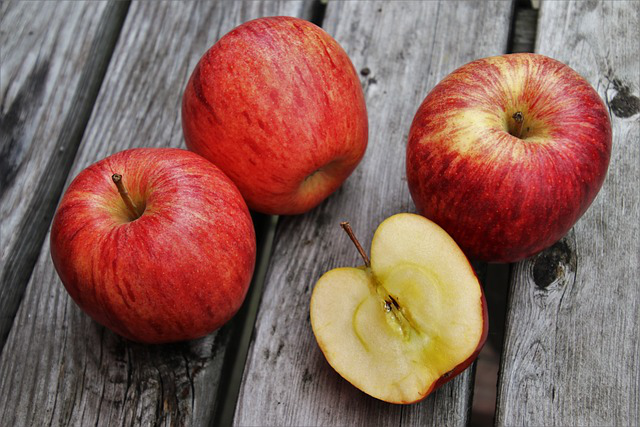
\includegraphics[width=0.24\textwidth]{apples.png}}
    \subfigure{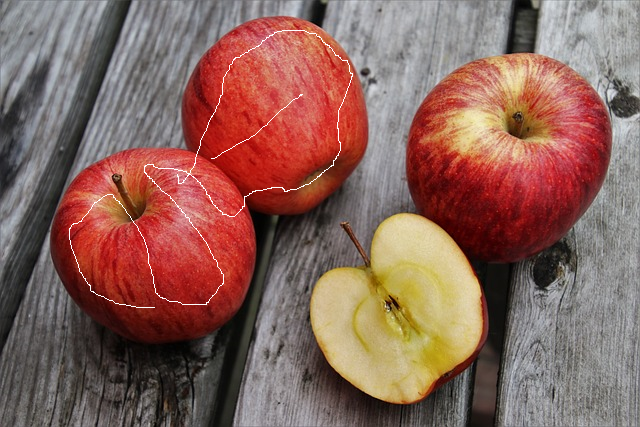
\includegraphics[width=0.24\textwidth]{apples_fore.png}}
    \subfigure{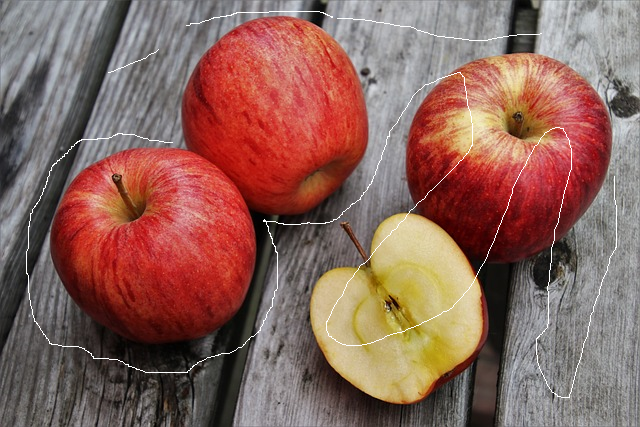
\includegraphics[width=0.24\textwidth]{apples_back.png}} \\
    \subfigure{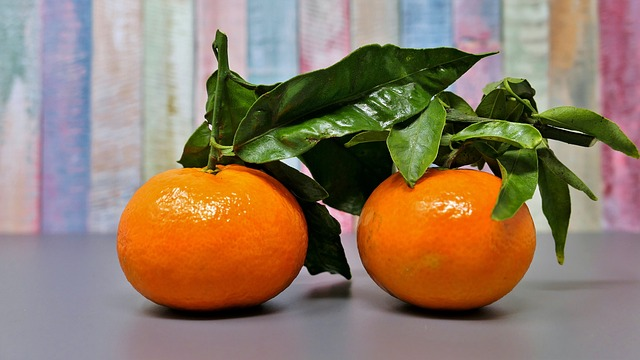
\includegraphics[width=0.24\textwidth]{mandarins.png}}
    \subfigure{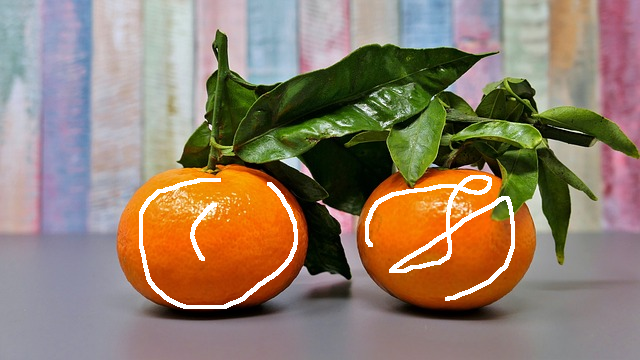
\includegraphics[width=0.24\textwidth]{mandarins_fore.png}}
    \subfigure{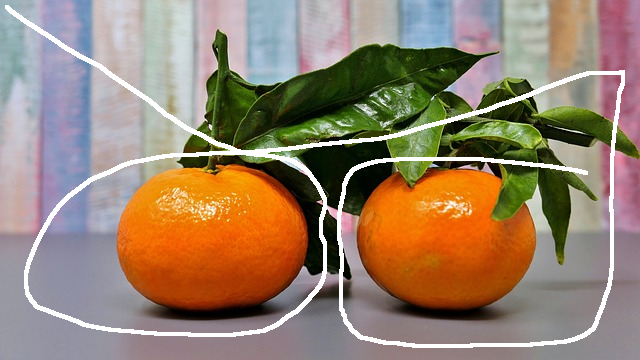
\includegraphics[width=0.24\textwidth]{mandarins_back.png}}
    \caption{Training datasets with foreground and background scribbles}
    \label{data}
\end{figure}

\begin{table}
    \centering
    \caption{Performance evaluation on the "Mandarins" dataset}
    \begin{tabular}{lll}
        \toprule
              & \multicolumn{2}{c}{IoU}                \\
        \cmidrule(r){2-3}
        Model & No Teacher              & With Teacher \\
        \midrule
        FICNN & 0.9152                  & 0.9345       \\
        Our   & 0.9422                  & 0.9592       \\
        \bottomrule
    \end{tabular}
    \label{exp}
\end{table}

\begin{figure}
    \centering
    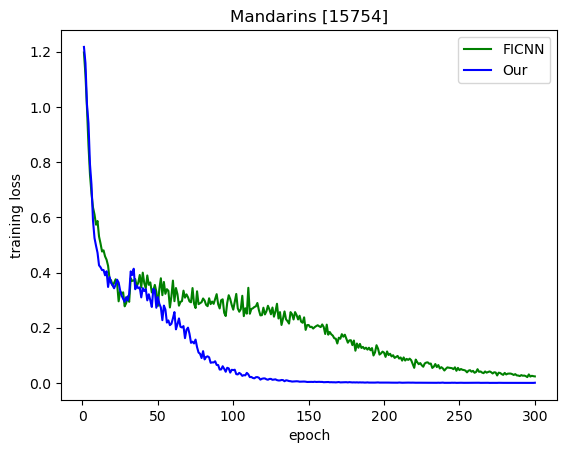
\includegraphics[width=0.65\textwidth]{training.png}
    \caption{Training loss on the "Mandarins" dataset.
        The spike at epoch 30 is explained by the change of the loss function.}
    \label{training}
\end{figure}

\begin{figure}
    \centering
    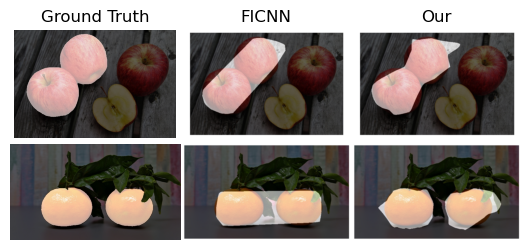
\includegraphics[width=0.65\textwidth]{resources/segmentation_result.png}
    \caption{Visual comparison of FICNN and our approach}
    \label{visual}
\end{figure}

In this study, we evaluated the performance of the proposed approach based on two datasets
extracted from scribbles presented on the Figure~\ref{data}.
The datasets "Apples" and "Mandarins" contain 3720 and 15774 labeled datapoints, respectively.

We compared our approach against a 3-layer FICNN (\cite{amos2017input}) with and without
a teacher network. The purpose of the teacher network is to provide both our composite network and FICNN
with the labels for the unlabeled pixels, since. The network can be arbitrarily complex or even omitted.

In the setting of scribble-based image segmentation, the amount of labeled pixels is usually low,
relatively to the size of the segmented image.
Therefore, as highlighted in the Table~\ref{exp}, the use of even a simple teacher
network leads to an increase in the quality of the resulting segmentation mask
without affecting the connectedness.
In our experiments, we employed a fully-connected network
with two hidden layers of 130 neurons each.

The training was performed jointly. In the Section~\ref{loss} we explain how the
loss function used for training is constructed.
We used Adam optimizer with a static learining rate of $10^{-4}$.
Each configuration was trained for 300 epochs with the batch size of 1500.
In each epoch, 1200 random datapoints from the dataset are combined with the input
in order to increase generalization abilities of the model by making it less prone to overfitting.

Our experiments show that our approach allows to achieve higher segmentation quality
as compared to the FICNN.
Moreover, due to the fact that our model performs segmentation only based
on the positional information of each pixel in the dataset, it is completely invariant to noise.

The Figure~\ref{visual} provides visual comparison of our model against FICNN.
We can see that our approach allows more flexibility.
However, further investigation is needed to determine the reason of having two path-connected
regions in the segmentation mask of the Mandarins dataset.
Our conjecture is that the model learns to preserve the connectedness
in the latent space despite the segmented objects being disconnected in the data space.

We can also see on the Figure \ref{training}, that our model converges faster than FICNN.

\subsection{Loss function}
\label{loss}

In order to perform joint training of both our model and the teacher network,
we introduce a loss function which evolves during the training process.
The base loss function is binary cross-enrtopy loss:

\[
    L(y_{t}, y, \hat{y}) = BCE(y_{t}, \hat{y}) + BCE(y, \hat{y})
\]

where $y_{t}$ and $y$ are the predictions of the teacher network and our model, respectively,
and $\hat{y}$ is the ground truth.

After 30 epochs, we add the mean squared error between the predictions of our model
and the rounded predictions of the teacher network.
Thus, the loss function evolves to the following form:

\[
    L(y_{t}, y, \hat{y}) = BCE(y_{t}, \hat{y}) + BCE(y, \hat{y}) + MSE(y, round(y_t))
\]

After 200 epochs, we require our model to match the predictions of the teacher model more by
omitting the rounding of its predictions and using $y_t$ unmodified.

\section{Conclusions}

We have developed a machine learning technique that enables the accurate
segmentation of images at a per-pixel level.
This approach has been extensively analyzed, and through mathematical proofs,
we have demonstrated that the decision space resulting from this technique
is path-connected. By imposing mathematical constraints on the network,
we are able to enhance the interpretability of the model's output and increase
its resilience against noise interference.
We further aim to expand the application of this method to a wider range of tasks
in order to create a more generalized model.
Additionally, we are keen on conducting further investigations to gain deeper
insights into the behavior of the model.

\bibliography{references.bib}

%%%%%%%%%%%%%%%%%%%%%%%%%%%%%%%%%%%%%%%%%%%%%%%%%%%%%%%%%%%%


\end{document}